\documentclass[a4paper, twoside]{report}
\usepackage[utf8]{inputenc}
\usepackage{graphicx}
\usepackage[colorlinks=true, allcolors=blue]{hyperref}
\graphicspath{{images/}}

\usepackage[a4paper,width=150mm,top=25mm,bottom=25mm,bindingoffset=6mm]{geometry}
\usepackage{fancyhdr}
\pagestyle{fancy}
\fancyhf{}
\fancyhead{}
\fancyhead[RO,LE]{Proyecto de Tesis}
\fancyfoot{}
\fancyfoot[LE,RO]{\thepage}
\fancypagestyle{plain}{}

\usepackage{amsmath}
\usepackage[colorinlistoftodos]{todonotes}
\usepackage{pgfgantt}
\renewcommand{\figurename}{Figura}

\title{Proyecto de Tesis}
\author{Franco Lianza}
\begin{document}

\begin{titlepage}

    \newcommand{\HRule}{\rule{\linewidth}{0.5mm}}

    \center
    
\includegraphics[width=0.4\textwidth]{university.jpg}\\[1cm]

    \textsc{\Large Maestr\'ia en Explotaci\'on de Datos y Gesti\'on del Conocimiento}\\[1.5cm]

    \makeatletter
    \HRule \\[0.6cm]
    {\huge \bfseries \@title}\\[0.4cm]
    \HRule \\[2cm]

    {\Large \@author}\\[3cm]

    {\large Abril 2022}\\[2cm]

    \vfill
\end{titlepage}
\newpage

\subsection*{Tema}
{\it Título del trabajo}

Clasificaci\'on de los digitos escritos en los telegramas de las elecciones
legislativas en Santa Fe mediante t\'ecnicas de adaptaci\'on de dominio.

\subsection*{Resumen}
{\it Resumen del área sobre la que se realizará el trabajo.}

La rama de {\it Computer Vision} se encarga desarrollar herramientas para
reconocer patrones complejos en im\'agenes en m\'ultiples dominios. Se ha
extendido exponencialmente a lo largo del tiempo, llegando a un punto en el
cual se pueden detectar todo tipo de objetos con una precisi\'on \'optima
\cite{szeliski2010computer}.

Las t\'ecnicas desarrolladas en el \'area precisan de un gran volumen de datos
para su entrenamiento. Esto implica que es de suma importancia de tener
disponibles las {\it labels} (etiquetas) de los datos que se van a utilizar
para entrenar los modelos. El etiquetado de los datos es una tarea costosa,
ineficiente y hasta a veces resulta inviable de realizar \cite{reis2022data}.

A\'un teniendo los {\it labels}, puede ocurrir que el {\it dataset} (conjunto
de datos) donde se va a utilizar el modelo resulte diferente al que se utilizó
para entrenarlo. Por mencionar, un modelo de detecci\'on de rostros entrenado
en una etnia demogr\'afica particular funcionar\'a de manera err\'onea si se lo
aplica a otra. Este fen\'onmeno se conoce como {\it dataset bias} o {\it
		dataset shift} (sesgo en los datos). Dicho de otra manera, un modelo entrenado
en un {\it dataset} puede no generalizar correctamente debido al {\it dataset
		bias}. Algunos autores afirman que el sesgo es un problema que no se puede
evitar al momento de crear un {\it dataset} \cite{khosla2012undoing}.

La detecci\'on de d\'igitos en los telegramas de elecciones en Argentina
podr\'ia llevarse a cabo mediante un modelo entrenado en {\it datasets} de
d\'igitos p\'ublicos como el {\it MNIST} \cite{lecun1998gradient}. Como no
existe una \'unica forma de escribir, el modelo estar\'a sesgado a reconocer
d\'igitos escritos de forma similar a los que se encontraban en el {\it
		dataset} de entrenamiento. No ser\'a capaz de generalizar lo aprendido en un
dominio distinto.

En trabajos anteriores, se aplican distorsiones al conjunto de entrenamiento
para aumentar la cantidad de datos de entrenamiento y de esta forma el modelo
pueda generalizar y aplicarse a los telegramas de elecciones de la Ciudad de
Buenos Aires \cite{Lamagna2016}. En el presente trabajo se utilizar\'an
t\'ecnicas referidas al {\it transfer learning}, espec\'ificamente de {\it
		domain adaptation} para resolver el problema.

El {\it transfer learning} (transferencia de aprendizaje) es un \'area del {\it
		machine learning} que se encarga de almacenar el conocimiento ganado en un
problema y aplicarlo a otro. {\it Domain adaptation} (adaptaci\'on de dominio)
consiste en la habilidad de aplicar un modelo entrenado en uno o mas dominios
de origen ({\it source domain}) en un uno distinto pero relacionado ({\it
		target domain}). La figura \ref{fig:mnist-to-svhn} muestra un ejemplo dos {\it
		datasets} de d\'igitos pero con dominios diferentes. Un modelo entrenado con
	{\it MNIST} no generalizar\'a al conjunto {\it SVHN} por m\'as que ambos sean
d\'igitos.

\begin{figure}[ht]
	\centering
	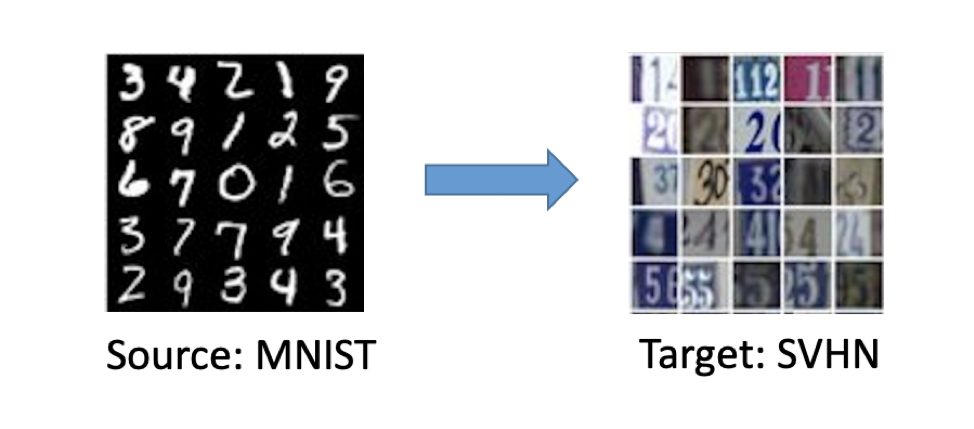
\includegraphics[width=0.6\textwidth]{mnist-to-svhn.png}
	\caption{Ejemplo dominios diferentes: MNIST y SVHN}
	\label{fig:mnist-to-svhn}
\end{figure}

\subsection*{Director o Tutor}
{\it El nombre del director o tutor de la tesis o trabajo, si éste ya
	hubiese aceptado la tarea.}

Dr. Leandro Bugnon

\subsection*{Motivación e importancia del campo}
{\it Explicar la o las motivaciones que llevan a realizar el trabajo planteado
	y su importancia.}

La principal motivaci\'on es obtener un modelo que, basado en un {\it dataset}
similiar ya etiquetado, pueda interpretar los d\'igitos de los telegramas de
las elecciones de Santa Fe sin necesitar el costoso proceso de etiquetar los
datos. De esta manera, el modelo podr\'ia utilizarse en futuras elecciones a
fin de automatizar la digitalizaci\'on de los mismos reduciendo
considerablemente los costos operacionales y reduciendo los posibles errores
humanos.

\subsection*{Problemas no resueltos}
{\it Problemas no resueltos detectados en el área y que el trabajo a realizar
	pretende resolver.}

La digitalizaci\'on de los telegramas de las elecciones sigue siendo de forma
manual, lo que genera lentitud y desconfianza en el proceso. Detectar los votos
de manera autom\'atica y reducir la intervenci\'on humana, aumentar\'a la
eficiencia de las elecciones y la confianza en ellas.

Por otra parte, cada una de las t\'ecnicas existentes de {\it domain
		adaptation} pretende aumentar el poder de generalizaci\'on del modelo de una
forma diferente. Debido a la variedad t\'enicas que existen, no es claro c\'ual
conviene utilizar en la digitalizaci\'on de los telegramas.

\subsection*{Objetivo del trabajo}
{\it Explicar claramente el objetivo del trabajo, especificando su alcance y limitaciones.}

El objetivo del trabajo consiste en desarrollar un m\'etodo para realizar
adaptaci\'on de dominio de un modelo aplicado a la digitalizaci\'on de los
telegramas de las elecciones legislativas de Santa Fe sin que necesite el
etiquetado de los mismos.

\subsection*{Requerimientos y desafíos}
{\it Requerimientos y desafíos que plantea el trabajo a realizar.}

Debido a que se posee tanto los datos como el poder de c\'omputo, el proyecto
presenta como principal desaf\'io analizar e implementar distintas t\'ecnicas
de {\it domain adaptation} a un modelo de reconocimiento de d\'igitos. Se
deber\'an estudiar diferentes conceptos de los cuales dependen las mismas, como
las {\it Generative Adversarial Networks (GANs)}
\cite{Tzeng_2017,ganin2016domain}.

\subsection*{Metodología}
{\it Metodología a emplear para el desarrollo del trabajo.}

Se har\'a revisi\'on del estado del arte para despu\'es continuar con el
preprocesamiento de los datos. Los telegramas ser\'an descargados desde la
\href{https://op.elecciones.gob.ar/telegramas/generales2021/}{p\'agina oficial
	del estado argentino}. Luego se extraer\'an los d\'igitos de los votos de cada
telegrama utilizando la librer\'ia {\it OpenCV} \cite{opencv_library}. Una vez
obtenido los d\'igitos, se realizar\'an ciclos de selecci\'on de t\'ecnica de
	{\it domain adaptation}, entrenamiento de distintas redes convolucionales
(LeNet \cite{lecun1998gradient}, ResNet \cite{he2016deep}, etc),
implementaci\'on de la adaptaci\'on y evaluaci\'on. Finalmente, se
seleccionar\'a el mejor modelo adaptado al problema.

\subsection*{Plan de Trabajo}
{\it Especificar las distintas tareas a realizar con los tiempos que se
	estime que deberían insumir.
	Indicar las fechas estimadas de inicio y finalización del trabajo.
}

El trabajo se realizar\'a a partir de las siguientes etapas:
\begin{itemize}
	\item \underline{Estudio del estado del arte}: estudiar las diferentes t\'ecnicas
	      de {\it domain adaptation}.
	\item \underline{Extracci\'on datos}: recolectar los telegramas
	      y extraer los d\'igitos de los votos.
	\item \underline{Limpieza de datos}: detectar votos incorrectos (por ejemplo
	      letras) y tratarlos para reducir lo m\'aximo posible el ruido
	      en los datos.
	\item \underline{Experimentaci\'on}: realizar ciclos de entrenamiento de modelos
	      y adaptarlos mediante alguna de las t\'ecnicas disponibles.
	\item \underline{Elaboraci\'on de reportes}: generar reportes que sinteticen los
	      experimentos realizados para compararlos.
	\item \underline{Redacci\'on de tesis}.
\end{itemize}

Se estima que el proyecto comienza en Agosto del 2022 y finaliza en Diciembre
del 2022. La figura \ref{fig:gantt} presenta el cronograma propuesto.

\begin{figure}[ht]
	\begin{center}

		\begin{ganttchart}[y unit title=0.4cm,
				y unit chart=0.5cm,
				vgrid,hgrid,
				title label anchor/.style={below=-1.6ex},
				title left shift=.05,
				title right shift=-.05,
				title height=1,
				progress label text={},
				bar height=0.7,
				group right shift=0,
				group top shift=.6,
				group height=.3]{1}{20}
			%labels
			\gantttitle{Agosto}{4}
			\gantttitle{Septiembre}{4}
			\gantttitle{Octubre}{4}
			\gantttitle{Noviembre}{4}
			\gantttitle{Diciembre}{4}\\
			\gantttitle{1}{1}
			\gantttitle{2}{1}
			\gantttitle{3}{1}
			\gantttitle{4}{1}
			\gantttitle{1}{1}
			\gantttitle{2}{1}
			\gantttitle{3}{1}
			\gantttitle{4}{1}
			\gantttitle{1}{1}
			\gantttitle{2}{1}
			\gantttitle{3}{1}
			\gantttitle{4}{1}
			\gantttitle{1}{1}
			\gantttitle{2}{1}
			\gantttitle{3}{1}
			\gantttitle{4}{1}
			\gantttitle{1}{1}
			\gantttitle{2}{1}
			\gantttitle{3}{1}
			\gantttitle{4}{1}\\

			%tasks
			\ganttbar{Estudio del estado del arte}{1}{6} \\
			\ganttbar{Extracci\'on de datos}{3}{4} \\
			\ganttbar{Limpieza de datos}{5}{6} \\
			\ganttbar{Esperimentaci\'on}{7}{12} \\
			\ganttbar{Elaboraci\'on de reportes}{12}{13} \\
			\ganttbar{Redacci\'on de tesis}{14}{20}

		\end{ganttchart}
	\end{center}
	\caption{Distribuci\'on de las tareas del proyecto.}
	\label{fig:gantt}
\end{figure}

\subsection*{Bibliograf\'ia}
{
	%Disable chapter command
	\renewcommand{\chapter}[2]{}
	\bibliographystyle{unsrt}
	\bibliography{refs}
}

\end{document}